% DPF 09 talk on strangeness in nucleon

\documentclass[10pt]{beamer}
\usepackage{amsmath}
\usefonttheme{professionalfonts} % using non standard fonts for beamer
\usefonttheme{serif} % default family is serif\
\usepackage{mathtools}
%\documentclass[12pt]{beamerthemeSam.sty}
\usepackage{epsf}
\usepackage{ulem}
\usepackage{array}
%\usepackage{pstricks}
%\usepackage[orientation=portrait,size=A4]{beamerposter}
\geometry{paperwidth=160mm,paperheight=120mm}
%DT favorite definitions
\def\LL{\left\langle}	% left angle bracket
\def\RR{\right\rangle}	% right angle bracket
\def\LP{\left(}		% left parenthesis
\def\RP{\right)}	% right parenthesis
\def\LB{\left\{}	% left curly bracket
\def\RB{\right\}}	% right curly bracket
\def\PAR#1#2{ {{\partial #1}\over{\partial #2}} }
\def\PARTWO#1#2{ {{\partial^2 #1}\over{\partial #2}^2} }
\def\PARTWOMIX#1#2#3{ {{\partial^2 #1}\over{\partial #2 \partial #3}} }

\def\rightpartial{{\overrightarrow\partial}}
\def\leftpartial{{\overleftarrow\partial}}
\def\diffpartial{\buildrel\leftrightarrow\over\partial}

\def\BI{\begin{itemize}}
\def\EI{\end{itemize}}
\def\BE{\begin{displaymath}}
\def\EE{\end{displaymath}}
\def\BEA{\begin{eqnarray*}}
\def\EEA{\end{eqnarray*}}
\def\BNEA{\begin{eqnarray}}
\def\ENEA{\end{eqnarray}}
\def\EL{\nonumber\\}
\def\BS{\bigskip}
\def\BC{\begin{center}}
\def\EC{\end{center}}
\def\BCC{\begin{columns}}
\def\ECC{\end{columns}}
\def\HC{\column{0.5\textwidth}}
\newcommand{\map}[1]{\frame{\frametitle{\textbf{Course map}}
\centerline{\includegraphics[height=0.86\paperheight]{../../map/#1.png}}}}
\newcommand{\wmap}[1]{\frame{\frametitle{\textbf{Course map}}
\centerline{\includegraphics[width=0.96\paperwidth]{../../map/#1.png}}}}

\newcommand{\etal}{{\it et al.}}
\newcommand{\gbeta}{6/g^2}
\newcommand{\la}[1]{\label{#1}}
\newcommand{\ie}{{\em i.e.\ }}
\newcommand{\eg}{{\em e.\,g.\ }}
\newcommand{\cf}{cf.\ }
\newcommand{\etc}{etc.\ }
\newcommand{\atantwo}{{\rm atan2}}
\newcommand{\Tr}{{\rm Tr}}
\newcommand{\dt}{\Delta t}
\newcommand{\op}{{\cal O}}
\newcommand{\msbar}{{\overline{\rm MS}}}
\def\chpt{\raise0.4ex\hbox{$\chi$}PT}
\def\schpt{S\raise0.4ex\hbox{$\chi$}PT}
\def\MeV{{\rm Me\!V}}
\def\GeV{{\rm Ge\!V}}

%AB: my color definitions
%\definecolor{mygarnet}{rgb}{0.445,0.184,0.215}
%\definecolor{mygold}{rgb}{0.848,0.848,0.098}
%\definecolor{myg2g}{rgb}{0.647,0.316,0.157}
\definecolor{abtitlecolor}{rgb}{0.0,0.255,0.494}
\definecolor{absecondarycolor}{rgb}{0.0,0.416,0.804}
\definecolor{abprimarycolor}{rgb}{1.0,0.686,0.0}
\definecolor{Red}           {cmyk}{0,1,1,0}
\definecolor{Grey}           {cmyk}{.7,.7,.7,0}
\definecolor{Lg}           {cmyk}{.4,.4,.4,0}
\definecolor{Blue}          {cmyk}{1,1,0,0}
\definecolor{Green}         {cmyk}{1,0,1,0}
\definecolor{Brown}         {cmyk}{0,0.81,1,0.60}
\definecolor{Black}         {cmyk}{0,0,0,1}

\usetheme{Madrid}


%AB: redefinition of beamer colors
%\setbeamercolor{palette tertiary}{fg=white,bg=mygarnet}
%\setbeamercolor{palette secondary}{fg=white,bg=myg2g}
%\setbeamercolor{palette primary}{fg=black,bg=mygold}
\setbeamercolor{title}{fg=abtitlecolor}
\setbeamercolor{frametitle}{fg=abtitlecolor}
\setbeamercolor{palette tertiary}{fg=white,bg=abtitlecolor}
\setbeamercolor{palette secondary}{fg=white,bg=absecondarycolor}
\setbeamercolor{palette primary}{fg=black,bg=abprimarycolor}
\setbeamercolor{structure}{fg=abtitlecolor}

\setbeamerfont{section in toc}{series=\bfseries}

%AB: remove navigation icons
\beamertemplatenavigationsymbolsempty
\title{
  \textbf {Rotational motion}\\
%\centerline{}
%\centering
%\vspace{-0.0in}
%\includegraphics[width=0.3\textwidth]{propvalues_0093.pdf}
%\vspace{-0.3in}\\
%\label{intrograph}
}

\author[W. Freeman] {Physics 211\\Syracuse University, Physics 211 Spring 2017\\Walter Freeman}

\date{\today}

\begin{document}

\frame{\titlepage}

\frame{\frametitle{\textbf{Announcements}}
\BI
\item{Next homework is due next Wednesday}
\item{Another short homework set will be due {\it on the day of your exam} -- 
it will be designed to help you study}
\item No office hours Friday (I'm traveling)
\EI
}

\frame{\frametitle{\textbf{Rotational motion, summarized}}
\Large
\BI
\item{Force diagrams: draw the entire object, and label at what point the forces act on them}
\item{Choose a pivot (for rotating things, choose the rotation axis}
\item{Newton's law for rotation: $\tau = I \alpha$}
\BI
\item{Applies separately for each rotating object}
\EI
\item{Sometimes you will also need $\vec F = m \vec a$}
\item{For static equilibrium problems: $\alpha = 0$}
\EI
}


\frame{\frametitle{\textbf{When do objects balance?}}
\Large
\BI
\item{Remember normal forces can only push, never pull}
\item{Think about what happens as something begins to tip}
\item{As an object topples over, its entire weight rests on the corner of the surface...}
\EI
}

\frame{\frametitle{\textbf{Agenda for today}}

\large You already know that rotational ideas correspond to translational ones:
\normalsize
\BS

\begin{center}
\begin{tabular}{l | l}

 \multicolumn{1}{c|}{\Large Translation} & \multicolumn{1}{c}{\Large Rotation} \\
 \\
\hline
\hline
 & \\
Position $\vec s$ & Angle $\theta$ \\
Velocity $\vec v$ & Angular velocity $\omega$ \\
Acceleration $\vec a$ & Angular acceleration $\alpha$ \\
 & \\
\hline
\hline
 & \\
Kinematics: $\vec s(t)\frac{1}{2}\vec at^2 + \vec v_0 t + \vec s_0$ & $\theta(t) = \frac{1}{2}\alpha t^2 + \omega_0 t + \theta_0$ \\
 & \\
\hline
\hline

 & \\
Force $\vec F$ & Torque $\vec \tau = \vec r \times \vec F$ \\
Mass $m$ & Moment of inertia $I$ \\
Newton's second law $\vec F_{\rm tot} = m \vec a$ & Newton's second law for rotation $\tau_{\rm tot} = I \alpha$ \\
 & \\

\hline
\hline
\end{tabular}
\BS
\large

\pause

You've also studied {\color{Red}kinetic energy} along with the {\color{Red}work-energy
theorem}. They have
rotational analogues as well.
\EC
}


\frame{\frametitle{\textbf {Rotational energy}}
\begin{center}
\begin{tabular}{l | l}

 \multicolumn{1}{c|}{\Large Translation} & \multicolumn{1}{c}{\Large Rotation} \\
 \\
\hline
\hline
Force $\vec F$ & Torque $\vec \tau = \vec r \times \vec F$ \\
Mass $m$ & Moment of inertia $I$ \\
Newton's second law $\vec F_{\rm tot} = m \vec a$ & Newton's second law for rotation $\tau_{\rm tot} = I \alpha$ \\

 & \\

\hline
\hline

 & \\
\color{Red}Kinetic energy $KE=\frac{1}{2}mv^2$ & \color{Red}Kinetic energy $KE=\frac{1}{2}I\omega^2$ \\
\color{Red}Work $W = \vec F \cdot \Delta \vec s$ & \color{Red}Work $W = \tau \Delta \theta$ \\
\color{Red}Power $P = \vec F \cdot \vec v$ & \color{Red}Power $P = \tau \omega$ \\
 & \\

\hline
\hline

 & \\

\hline
\end{tabular}
\BS

\large

Rotational kinetic energy and the rotational work-energy theorem
work like their translational counterparts.

\end{center}
}

\frame{\frametitle{\textbf{Rotational kinetic energy}}

\Large

There is also kinetic energy associated with rotation, too! (The pipe
problem from HW6...)

$$KE_{\rm rot} = \frac{1}{2}I\omega^2$$

\large

This is what we would expect, based on $KE_{\rm trans} = \frac{1}{2}mv^2$:

\BI
\item Moment of inertia $I$ is the rotational analogue of mass
\item Angular velocity $\omega$ is the rotational analogue of velocity
\EI
}



\frame{

\Large
\BCC
\HC
Suppose I release a Yo-Yo whose string has a length $h$. How fast will its center be moving
when it runs out of string?
\HC
\BC
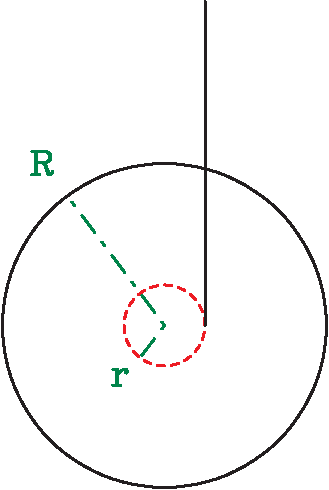
\includegraphics[width=0.4\textwidth]{yoyo-diagram-crop.pdf}
\EC
\ECC
\BS
\BS

\color{A}A: $v_f < \sqrt{2gh}$, because the tension in the string slows it down \\
\color{B}B: $v_f < \sqrt{2gh}$, because part of the GPE is required to make the Yo-Yo spin \\
\color{C}C: $v_f = \sqrt{2gh}$, by the conservation of energy \\
\color{D}D: $v_f > \sqrt{2gh}$, because the spinning disk speeds it up \\
}

\frame{
\large
{\color{C} Answer C} is what we get if there is no string. (We already know how to do that.)

\pause
\BCC
\HC
{\color{A} Answer A} makes sense; in a force diagram for the Yo-Yo, the tension
means that the net downward force is less than $mg$.
\HC
\BC
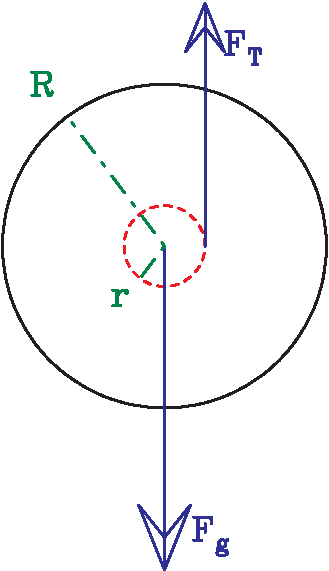
\includegraphics[width=0.4\textwidth]{yoyo-diagram-forces-crop.pdf}
\EC
\ECC

\pause
\BS

{\color{B} Answer B} makes sense as well, though: if the Yo-Yo spins as it falls,
then {\bf some energy is required to make it spin}, leaving less available
energy for translational kinetic energy.

\BS

We'll analyze this using energy methods. 

}


\frame{\frametitle{\textbf{The work done by tension}}
\large
We know the work-energy theorem for translational motion (for constant $\vec F$):

$$W_{\rm trans} \equiv \Delta \frac{1}{2}mv^2 = \vec F \cdot \Delta \vec s$$

\BS

Replacing $m$, $\vec F$, $\vec s$, and $v^2$ with their rotational counterparts, we get:

\BS
$$W_{\rm rot} \equiv \Delta \frac{1}{2}I\omega^2 = \tau \Delta \theta $$

\BS

This is the {\it rotational work-energy theorem.}
}

\frame{\frametitle{\textbf{The work done by tension}}

\Large
Which is true regarding the work done by tension here?
\BS
\Huge

\color{A}A: $W_{\rm total} = 0$ \\
\color{B}B: $W_{\rm trans} > 0, W_{\rm rot} > 0$ \\
\color{C}C: $W_{\rm trans} < 0, W_{\rm rot} > 0$ \\
\color{D}D: $W_{\rm trans} > 0, W_{\rm rot} < 0$ \\
\color{E}E: $W_{\rm trans} < 0, W_{\rm rot} < 0$ \\
\pause

\BS
\Large
\color{Black}
The string makes the Yo-Yo fall more slowly (negative translational work),
but makes it spin (positive rotational work). That means {\color{C}Answer C}
is correct. What about {\color{A}Answer A}?
}

\frame{\frametitle{\textbf{The work done by tension}}

\large


\BS\BS \pause

Rotational work: $W_{\rm rot} = \tau \Delta \theta$

\pause\BS

If the Yo-Yo falls a distance $h$, it turns through a (positive!) angle 
given by $\Delta \theta = h/r $.

\BS

The torque applied by the tension is $\tau = Tr$ (positive!).

\pause

\BS\BS
{\color{Red} Rotational work: $W_{\rm rot} = \tau \Delta \theta = Tr(h/r) = Th$.}\\
{\color{Blue}Translational work: $W_{\rm trans} = \vec F \cdot \Delta \vec s =-Th$.}
\BS
\pause

$\rightarrow$ The {\color{Red} total work done by tension here is zero.} (We could have guessed that!)
}

\frame{\frametitle{\textbf{Conservation of energy, including rotation}}

\Large
$$ {\rm PE_i} + \frac{1}{2}mv_i^2 + \frac{1}{2}I\omega_i^2 + W_{\rm NC} = 
{\rm PE_f} + \frac{1}{2}mv_f^2 + \frac{1}{2}I\omega_f^2 $$

\Large\BS

Which expression will let us find the velocity of the Yo-Yo at the bottom?

\begin{align*}
&\color{A}\rm A:& \color{A}mgh - Th &\color{A}= \color{A}\frac{1}{2}mv_f^2 + \frac{1}{2} I\omega_f^2 \\\BS
&\color{B}\rm B:&\color{B} mgh + \frac{1}{2}mv_i^2 &\color{B}= \frac{1}{2}mv_f^2 + \frac{1}{2} I\omega_f^2 \\\BS
&\color{C}\rm C:&\color{C} mgh &\color{C}= \frac{1}{2}mv_f^2  \\\BS
 &\color{D}\rm D:&\color{D} mgh &\color{D}= \frac{1}{2}mv_f^2 + \frac{1}{2} I\omega_f^2 \\\BS
\end{align*}
}

\frame{\frametitle{\textbf{What about rolling objects?}}

\large
In the Yo-Yo problem, we saw that:

\BI
\item Tension did positive rotational work (it made the Yo-Yo spin faster)
\item Tension did negative translational work (it made the Yo-Yo move more slowly)
\item ... the {\bf net work done by tension was zero}.
\EI

This happened because the string was stationary, and thus enforced $a=\pm \alpha r$.
This is also true in {\color{Red}rolling motion}.
}


\frame{\frametitle{\textbf{An object rolling down a hill}}
\Large

\BC
Consider first a ball sliding down a hill without friction.
\EC
\BCC
\HC
\BC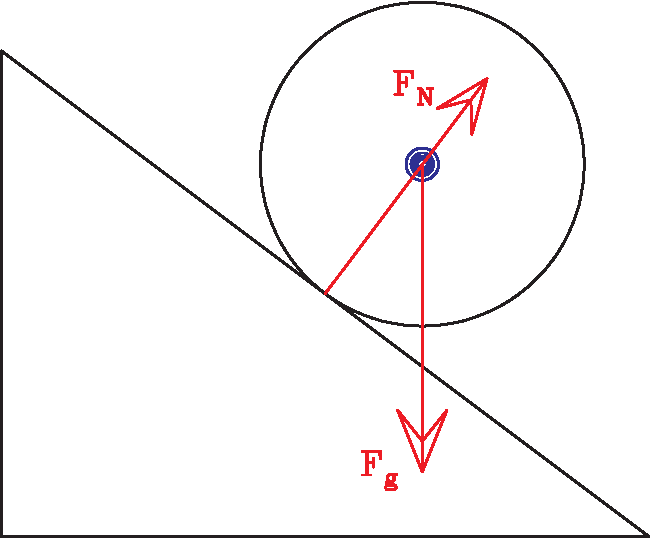
\includegraphics[width=0.8\textwidth]{hill-crop.pdf}\EC
\HC
Which of these forces applies a torque to the ball?

\BS
\color{A}A: Just the normal force \\
\color{B}B: Just gravity \\
\color{C}C: Both of them \\
\color{D}D: Neither of them \\
\ECC

\BS

\BC
\pause
Friction is required to make the ball spin!
\EC
}

\frame{\frametitle{\textbf{An object rolling down a hill}}
\Large

\BC
If the ball {\it rolls without slipping...}
\EC
\BCC
\HC
\BC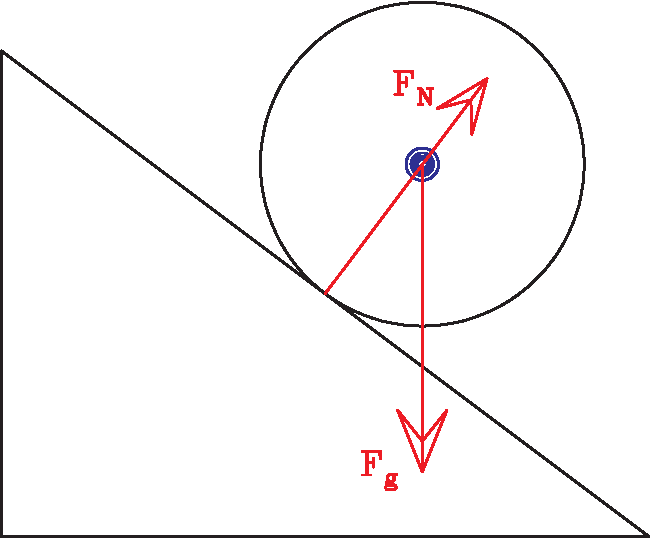
\includegraphics[width=0.8\textwidth]{hill-crop.pdf}\EC
\HC
\large
What is true about the frictional force?

\BS
\color{A}A: Static friction points down the ramp \\
\color{B}B: Static friction points up the ramp \\
\color{C}C: Kinetic friction points down the ramp \\
\color{D}D: Kinetic friction points up the ramp \\
\color{E}E: There is no friction
\ECC

\BS

}


\frame{\frametitle{\textbf{An object rolling down a hill}}
\Large

\BC
If the ball {\it rolls without slipping...}
\EC
\BCC
\HC
\BC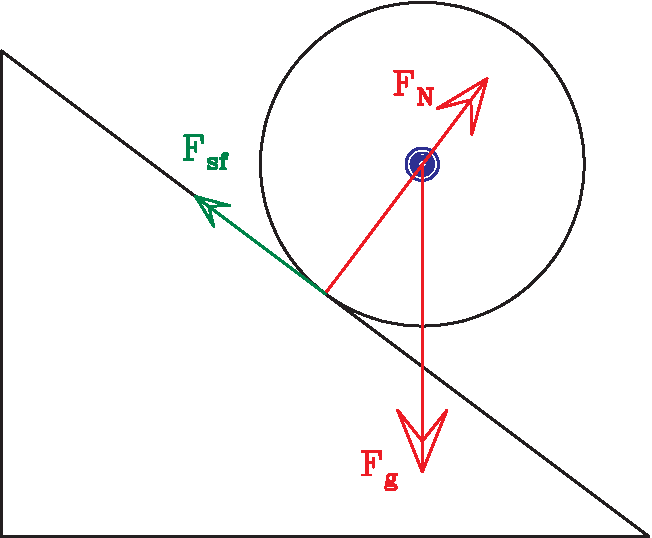
\includegraphics[width=0.8\textwidth]{hill-2-crop.pdf}\EC
\HC
\large
What is true about the frictional force?

\BS
\color{A}A: Static friction points down the ramp \\
\color{B}B: Static friction points up the ramp \\
\color{C}C: Kinetic friction points down the ramp \\
\color{D}D: Kinetic friction points up the ramp \\
\color{E}E: There is no friction
\ECC

\BS

\BC
The point of contact would {\color{Red} slide downward} without friction, so friction 
points {\color{Red} back up the ramp}. This is static friction since the ball 
doesn't slide.
\EC




}

\frame{\frametitle{\textbf{Energy rolling down a hill}}

\large

Static friction {\color{Red} does no total work} on the ball:
\BI
\item it reduces the translational kinetic energy $\frac{1}{2}mv^2$
\item it increases the rotational kinetic energy $\frac{1}{2}I\omega^2$
\item ... but it leaves the sum $\frac{1}{2}mv^2 + \frac{1}{2}I\omega^2$ unchanged
\EI

\BS

\BCC
\HC
\BC
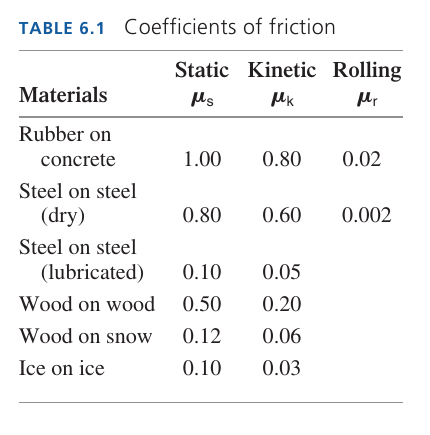
\includegraphics[width=0.8\textwidth]{mu-table.png}

\scriptsize (From {\it Physics for Scientists and Engineers}, Knight, 3rd ed.)
\EC
\HC
This is not {\it quite} true -- rolling friction does exist. There is 
a little bit of overall negative work done as tires flex and so on, but it is small.
\ECC
}



\frame{
\Large

This means that we can use our standard expression for conservation of energy
for rolling objects, {\it ignoring} the force of static friction required to keep them
from slipping:

$$ {\rm PE}_i + \frac{1}{2}mv_i^2 + \frac{1}{2}I\omega_i^2 + W_{\rm NC} = 
{\rm PE}_f + \frac{1}{2}mv_f^2 + \frac{1}{2}I\omega_f^2 $$

How fast will each object ($I = \lambda mr^2$) be traveling at the bottom
of the ramp?}

\frame{
\Large

How high must I start the ball for it to make it around the loop?

}

\frame{\frametitle{\textbf{Rotational dynamics and power}}

\Large

If $W = \tau \Delta \theta$, then $P = \tau \omega$.

\BS

If I want to supply a power $P$, I can either exert a large torque at a 
small angular velocity, or a small torque at a large angular velocity.

\BS
\BS

$\rightarrow$ bicycle demonstration!
}


\frame{\frametitle{\textbf{Angular momentum}}
\begin{columns}
\column{0.5\textwidth}
\color{Grey}
\Large
\centerline{Translational motion}
\normalsize
\BI
{\color{Red}
\item{Moving objects have momentum}
\item{$\vec p = m \vec v$}
\item{Momentum conserved if there are no external forces}}
\EI
\column{0.5\textwidth}
\color{Grey}
\Large
\centerline{Rotational motion}
\normalsize
\BI
{\color{Blue}
\item{Spinning objects have angular momentum $L$}
\item{$L = I \omega$}
\item{Angular momentum conserved if no external torques}}
\EI
\end{columns}

\bigskip
\bigskip

\Large
\color{Red}

$\rightarrow$ $L = I \omega = $ constant; analogue to conservation of momentum

}

\frame{\frametitle{\textbf{Conservation of angular momentum}}
\large
We saw that the conservation of momentum was valuable mostly in two sorts of situations:

\BI
\item{Collisions: two objects strike each other}
\item{Explosions: one object separates into two}
\EI

There is a third common case for conservation of angular momentum:

\BI
\item{Collisions: a child runs and jumps on a merry-go-round}
\item{Explosions: throwing a ball off-center}
\item{{\color{Red}A spinning object changes its moment of inertia}}
\EI

\pause
\bigskip

This last happens because moment of inertia depends on {\it how the mass is distributed}, not just how much there is!
}

\frame{\frametitle{\textbf{Conservation of angular momentum}}

\Large
\BC

These problems are approached in exactly the same way as conservation of 
{\it linear} momentum problems: write down expressions for $L_i$ and $L_f$ 
and set them equal (if there are no external torques).

\Huge

$$L = I \omega$$

$$\sum L_i=\sum L_f$$ \\

\EC
}


\frame{\frametitle{\textbf{Conservation of angular momentum}}
\Large
If I kept the mass of the Earth the same, but enlarged it so that it had twice
the diameter, how long would a day be?

\BS

(Remember, the total angular momentum, $L=I\omega$, stays the same)

\BS
\BS

\Huge

\color{A}A: 6 hours\\
\color{B}B: 12 hours\\
\color{C}C: 24 hours\\
\color{D}D: 48 hours\\
\color{E}E: 96 hours\\
}


\frame{\frametitle{\textbf{Angular momentum of a single object}}

\large

A single object moving in a straight line also has angular momentum.

\Huge
$$L = mv_\perp r = mvr_\perp$$
\large

Example: A child of mass $m$ runs straight east and jumps onto a merry-go-round of mass $M$ and radius $r$,
landing $2/3$ of the way toward the outside. If she lands on the south edge,
how fast will it be turning once she lands?

\BS

We'll do this together on the document camera.

}

\frame{\frametitle{\textbf{Angular momentum demonstrations}}

\Large

Can a spinning person change their moment of inertia?

\pause\BS\BS

Can a spinning person exchange angular momentum with a spinning object?



\end{document}

\end{document}
